\documentclass{book}
% see also:
% https://plmlatex.math.cnrs.fr/6975232963dbybcdhpktwf

% Language setting
% Replace `english' with e.g. `spanish' to change the document language
\usepackage[english]{babel}

% Set page size and margins
% Replace `letterpaper' with`a4paper' for UK/EU standard size
\usepackage[letterpaper,top=2cm,bottom=2cm,left=3cm,right=3cm,marginparwidth=1.75cm]{geometry}

% Useful packages
\usepackage{amsmath}
\usepackage{graphicx}
\usepackage[colorlinks=true, allcolors=blue]{hyperref}
\usepackage{bbold}
\usepackage{bbm, dsfont}
\usepackage{xcolor}

%% biblio
\usepackage[backend=biber,style=apa,refsegment=chapter]{biblatex}
\addbibresource{sample.bib}

%% Images path
\graphicspath{{Imagens/}{./}}

% Capa
\title{Mecânica, difusão e elementos finitos para pessoas como nós :)}
\author{Lúcio, Paulo de Souza, Tárique que não vale nada}

\date{O dia que nunca terminou}

\makeindex

% ======================
\begin{document}
	
	% Preâmbulo
	\maketitle	
	\chapter*{Agradecimentos}
Só deus sabe como ta a cabeça do palhaço

\chapter*{Dedicatória}
ao medonho por ter juntado tanta mente perturbada no mesmo lugar :)

\newpage
	\tableofcontents	
	\listoffigures
	\listoftables

	% Capítulos
	\chapter{Introdução}

O presente trabalho se trata do desenvolvimento de uma ferramenta baseada um métodos numéricos, seu uso é variado mas inicialmente é voltado para a aproximação de soluções de problemas multi-física, isto é, mecânica linear e não-linear, difusão de Fick, propagação de ondas, entre outros que ainda não foram implementados. A biblioteca  é o resultado de um trabalho e minha participação foi mais voltada para módulos de mecânica, mas muitos módulos são usados por todos os tipos de problema, então meu trabalho aborde pontos mais e não só o meu assunto foco.
Os módulos de solução são baseadas em métodos discretos (Finite Element Method - FEM) e semi-analíticos (Semi-Analytical Finite Elements - SAFE) presentes nas diversas bibliotecas escritas em MATLAB que juntas formam uma poderosa ferramenta de soluções numéricas. Essas bibliotecas estão divididas em três grandes grupos: Pre-Processamento, Processamento e Pós-Processamento. 
 
A implementação das rotinas de solução de mecânica linear e não-linear.
	
	\chapter{Revisão de matemática e física}\label{ch:rev}

\section{Notação}

\section{Vetores e tensores}

\section{Gradiente, divergente e rotacional}
{%\color{red}
	Muitas equações governantes da mecânica estrutural incluem a derivada de uma variável de campo em relação às coordenadas espaciais. Aqui, um "campo" refere-se a uma função no espaço, como a temperatura ou o deslocamento de uma estrutura. A variável de campo pode ser um escalar, vetor ou tensor. Portanto, é útil definir claramente o operador gradiente usando a notação tensorial.
	
	O operador gradiente é definido como um vetor (ou tensor de ordem 1) da seguinte forma:
	\begin{equation}
		\vec{\nabla} = e_i \frac{\partial}{\partial x_i}, \tag{1.23}
	\end{equation}
	\begin{equation}
		\vec{\nabla} \phi = \text{grad} \, \phi = e_i \frac{\partial \phi}{\partial x_i}, \tag{1.24}
	\end{equation}
	onde $e_i$ são os vetores base.
	
	Por exemplo, o gradiente de um campo escalar, $\phi(x)$, pode ser escrito como:
	\begin{equation}
		\frac{\partial \phi}{\partial x_i},
	\end{equation}
	que é um vetor. O gradiente de um campo vetorial, $u(x)$, pode ser definido como:
	\begin{equation}
		\vec{\nabla} u = e_i \frac{\partial u_j}{\partial x_i} e_j = \frac{\partial u_j}{\partial x_i},
	\end{equation}
	onde o gradiente de um vetor é um tensor de ordem 2.
	
	Para conveniência notacional, a vírgula subscrita será frequentemente usada para representar o gradiente, ou seja, $v_{i,j} = \frac{\partial v_i}{\partial x_j}$.
	
	---
	
	A seguinte divergência é definida para que o gradiente de um vetor produza uma quantidade escalar:
	\begin{equation}
		\vec{\nabla} \cdot u = e_i \frac{\partial u_i}{\partial x_i} = \frac{\partial u_1}{\partial x_1} + \frac{\partial u_2}{\partial x_2} + \frac{\partial u_3}{\partial x_3}. \tag{1.25}
	\end{equation}
	
	O operador de Laplace pode ser definido usando o produto interno de dois operadores gradientes como:
	\begin{equation}
		\vec{\nabla}^2 = \vec{\nabla} \cdot \vec{\nabla} = e_i \frac{\partial}{\partial x_i} \left( \frac{\partial}{\partial x_j} e_j \right),
	\end{equation}
	\begin{equation}
		\vec{\nabla}^2 = \frac{\partial^2}{\partial x_1^2} + \frac{\partial^2}{\partial x_2^2} + \frac{\partial^2}{\partial x_3^2}. \tag{1.26}
	\end{equation}
	
	---
	
	\emph{Exemplo 1.4 (Divergência de um Tensor de Tensões)}
	
	Seja $\sigma$ o tensor de tensões dado na Eq. (1.5). O equilíbrio de forças de um componente infinitesimal pode ser escrito como:
	\begin{equation}
		\vec{\nabla} \cdot \sigma = 0.
	\end{equation}
	
	Escreva a equação de equilíbrio de forças na forma de componentes.
	
	\textbf{Solução:} Substituindo o vetor $u$ na Eq. (1.26) pelo tensor de tensões, a divergência do tensor de tensões torna-se:
	\begin{equation}
		(\vec{\nabla} \cdot \sigma)_j = \frac{\partial \sigma_{ij}}{\partial x_i}.
	\end{equation}
	
	Expandindo a equação acima para todos os componentes e definindo a divergência como igual a zero, obtemos as seguintes equações diferenciais para o equilíbrio:
	\begin{equation}
		\frac{\partial \sigma_{11}}{\partial x_1} + \frac{\partial \sigma_{21}}{\partial x_2} + \frac{\partial \sigma_{31}}{\partial x_3} = 0,
	\end{equation}
	\begin{equation}
		\frac{\partial \sigma_{12}}{\partial x_1} + \frac{\partial \sigma_{22}}{\partial x_2} + \frac{\partial \sigma_{32}}{\partial x_3} = 0,
	\end{equation}
	\begin{equation}
		\frac{\partial \sigma_{13}}{\partial x_1} + \frac{\partial \sigma_{23}}{\partial x_2} + \frac{\partial \sigma_{33}}{\partial x_3} = 0.
	\end{equation}
	
	Será mostrado posteriormente que o tensor de tensões é simétrico, i.e., $\sigma_{12} = \sigma_{21}$, $\sigma_{23} = \sigma_{32}$ e $\sigma_{13} = \sigma_{31}$.
}
\section{Só uma pincelada sobre tensão e deformação}

\section{Teoremas integrais}
{%\color{red}
	Muitas equações na mecânica dos sólidos são expressas em termos de equações diferenciais. Por exemplo, o equilíbrio de forças de um componente infinitesimal pode ser expresso em termos de equações diferenciais parciais. Como essas equações diferenciais são satisfeitas em todos os pontos do domínio de uma estrutura, elas são integradas sobre todo o domínio; o resultado é uma equação integral. Nesta seção, são introduzidos diversos teoremas úteis na derivação das equações integrais da mecânica dos sólidos. A demonstração de cada teorema está fora do escopo deste texto. Leitores interessados podem consultar o texto de Hildebrand CITAR[3].
	
	\subsection*{Teorema da Divergência}
	
	O teorema da divergência é um caso especial do teorema de Green para um campo tensorial. O teorema da divergência relaciona uma integral de domínio a uma integral de contorno em torno do domínio. Seja $\Omega$ um domínio delimitado por $\Gamma$. Se um tensor $A$ tem derivadas parciais contínuas no domínio, a integral da divergência de $A$ no domínio pode ser convertida em uma integral sobre o contorno, como:
	\begin{equation}
		\iint_\Omega (\nabla \cdot A) \, d\Omega = \int_\Gamma (n \cdot A) \, d\Gamma, \tag{1.28}
	\end{equation}
	onde $n$ é o vetor unitário normal para fora da superfície $\Gamma$. 
	
	Uma variante do teorema da divergência é o teorema do gradiente, no qual o produto interno é substituído pelo produto diádico:
	\begin{equation}
		\iint_\Omega (\nabla A) \, d\Omega = \int_\Gamma (n \otimes A) \, d\Gamma.
	\end{equation}
	
	\subsection*{Teorema de Transporte de Reynolds}
	
	O teorema de transporte de Reynolds está relacionado à derivada temporal de uma equação integral sobre um domínio no qual tanto o integrando quanto o domínio variam com o tempo. Considere integrar $f = f(x, t)$ sobre o domínio dependente do tempo, $\Omega(t)$, que é delimitado por $\Gamma(t)$. Então, a derivada temporal da integral de $f(x, t)$ sobre o domínio $\Omega(t)$ pode ser expressa como:
	\begin{equation}
		\frac{d}{dt} \iint_{\Omega(t)} f \, d\Omega = \iint_{\Omega(t)} \frac{\partial f}{\partial t} \, d\Omega + \int_{\Gamma(t)} (n \cdot v) f \, d\Gamma, \tag{1.29}
	\end{equation}
	onde $n(x, t)$ é o vetor normal unitário para fora do contorno, e $v(x, t)$ é a velocidade do contorno. O primeiro termo do lado direito (RHS) é chamado de derivada parcial, e o segundo termo é chamado de termo convectivo. Note que a integral no lado esquerdo (LHS) depende apenas do tempo, portanto, a derivada total é usada.
	
	\subsection*{Integração por Partes}
	
	A integração por partes é um teorema que relaciona a integral do produto de funções à integral de suas derivadas e antiderivadas. No caso unidimensional, se $u(x)$ e $v(x)$ são duas funções continuamente diferenciáveis no domínio $(a, b)$, a integração por partes pode ser escrita como:
	\begin{equation}
		\int_a^b u'(x) v(x) \, dx = \big[ u(x) v(x) \big]_a^b - \int_a^b u(x) v'(x) \, dx.
	\end{equation}
	
	Esta relação pode ser estendida para o caso bidimensional ou tridimensional. Seja $\Omega$ o domínio da integral com contorno $\Gamma$. Então, a integração por partes pode ser escrita como:
	\begin{equation}
		\iint_\Omega \frac{\partial u}{\partial x_i} v \, d\Omega = \int_\Gamma u v n_i \, d\Gamma - \iint_\Omega u \frac{\partial v}{\partial x_i} \, d\Omega,
	\end{equation}
	onde $n_i$ são os componentes do vetor normal unitário para fora do contorno $\Gamma$. Substituindo a função escalar $v$ na fórmula acima por um vetor $v_i$ e somando sobre $i$, obtemos a seguinte fórmula vetorial:
	\begin{equation}
		\iint_\Omega (\nabla u \cdot v) \, d\Omega = \int_\Gamma (u v \cdot n) \, d\Gamma - \iint_\Omega u (\nabla \cdot v) \, d\Omega. \tag{1.30}
	\end{equation}
	
	Substituindo $u = 1$ na fórmula acima, o teorema da divergência (Eq. 1.28) pode ser obtido. Para o propósito da mecânica dos contínuos, a seguinte identidade de Green pode ser derivada substituindo $v$ por $\nabla v$ na fórmula anterior:
	\begin{equation}
		\iint_\Omega (\nabla u \cdot \nabla v) \, d\Omega = \int_\Gamma (u \nabla v \cdot n) \, d\Gamma - \iint_\Omega u (\nabla^2 v) \, d\Omega. \tag{1.31}
	\end{equation}
	
	Uma das razões importantes para usar a integração por partes é relaxar o requisito de diferenciabilidade. Na fórmula acima, por exemplo, o lado direito (RHS) exige que $v(x)$ seja uma função duas vezes diferenciável, enquanto o lado esquerdo (LHS) está bem definido com a derivada parcial de primeira ordem de $v(x)$. O requisito adicional de diferenciabilidade foi transferido para $u(x)$.
	
	\emph{Exemplo 1.5 (Teorema da Divergência)}
	
	Integre $ \int_S F \cdot n \, dS $, onde $F$ é um campo vetorial dado por $F = 2x e_1 + y^2 e_2 + z^2 e_3$, e $S$ é a área da superfície da esfera unitária $(x^2 + y^2 + z^2 = 1)$, cujo vetor normal unitário é $n$.
	
	\textbf{Solução:} Usando o teorema da divergência:
	\begin{equation}
		\int_S F \cdot n \, dS = \iint_\Omega (\nabla \cdot F) \, d\Omega,
	\end{equation}
	\begin{equation}
		\iint_\Omega (\nabla \cdot F) \, d\Omega = \iint_\Omega \left( 2 + 0 + 0 \right) \, d\Omega = 2 \iint_\Omega 1 \, d\Omega = 2 \cdot \frac{4\pi}{3} = 8\pi / 3.
	\end{equation}
}

\section{Problema de valor sobre o contorno}

\section{Principio da miníma energia potencial}

\section{Principio dos trabalhos virtuais}

%% referencias
\nocite{malvern1969introduction}
\nocite{boresi2002advanced}
\printbibliography[heading=subbibliography,segment=\therefsegment]

	
	\chapter{Cinemática do Contínuo}
\section{Introdução}
Descrição da mudança geométrica de um meio, e eras isso.

\section{Mapeamento do Deslocamento}
Para descrever mudanças geométricas em um meio contínuo é necessário fazer o mapeamento do deslocamento dos pontos dentro do domínio. O corpo em estudo é interpretado como um conjunto de partículas que inicialmente ocupam uma posição inicial $\mathbf{X}$, no momento $t_0$, que formam uma configuração de referência $C_0$ onde o corpo ainda não sofreu nenhum tipo de alteração. Após o corpo sofrer as alterações externas que mudaram sua geometria, as partículas ocupam novas posições em $\mathbf{x}$ no momento $t$ que formam uma configuração deformada $C$. O mapeamento do deslocamento é a equação que descreve a mudança de posição dessas partículas de um estado para o outro. Se a equação descreve a mudança do estado \textbf{indeformado} para o \textbf{deformado} é dado o nome de descrição \textit{Lagrangiana}, se ela descreve a mudança do estado \textbf{deformado} para o \textbf{indeformado} é dado o nome de descrição \textit{Euleriana}. 

O conjunto de pontos das partículas denominado por $\mathbf{X}$ na descrição \textit{Lagrangiana} é chamado de \textit{coordenadas materiais} e são usadas para descrever como o geometria de um corpo sólido muda após a aplicação de cargas externas, por esse motivo é usado na mecânica dos sólidos. O conjunto de pontos das partículas denominado por $\mathbf{x}$ na descrição \textit{Euleriana} é chamado de \textit{coordenadas espaciais} e são usadas para descrever como as propriedades dentro de um volume de controle mudam após a aplicação de condições de contorno, por esse motivo é usado na mecânica dos fluidos.

As equações que descrevem a mudança do grupo de coordenadas $\mathbf{X}$ para $\mathbf{x}$ pode ser representado por

\begin{equation}
	\mathbf{x} = \chi(\mathbf{X}, t),
\end{equation}

\begin{equation}
	\chi(\mathbf{X}, t_0) = \mathbf{X}.
\end{equation}

%\begin{figure}
%	\centering
%	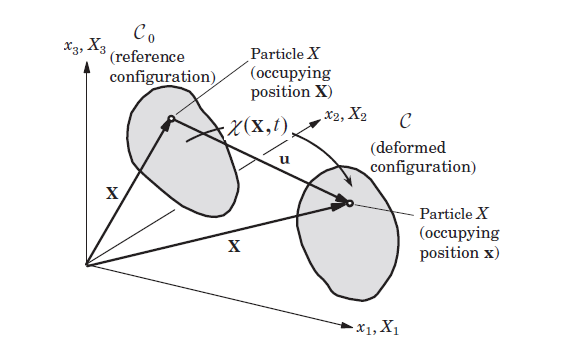
\includegraphics[width=0.6\linewidth]{fig_3-3-1_Reddy.png}
%	\caption{Mapeamento do Deslocamento}
%	\label{fig:my_label}
%\end{figure}

\subsection{Campo de Deslocamento}
O deslocamento dos pontos são a diferença entre as coordenadas das duas configurações do meio contínuo, como estamos falando de mecânica dos sólidos, daqui pra frente usaremos a descrição \textit{Lagrangiana} para montar as equações. Assim o deslocamento pode ser escrito como uma função das coordenadas \textit{materiais}

\begin{equation}
	\mathbf{u}(\mathbf{X}, t) = \mathbf{x}(\mathbf{X}, t) - \mathbf{X}.
	\label{dispX}
\end{equation}

%\begin{figure}
%	\centering
%	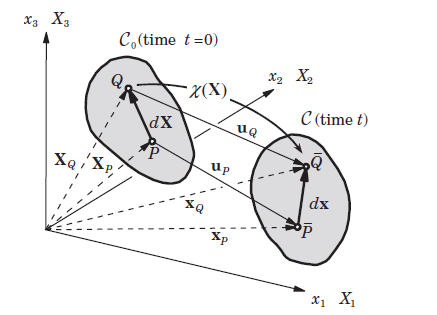
\includegraphics[width=0.6\linewidth]{fig_3-3-3_Reddy.png}
%	\caption{Campo de Deslocamento}
%	\label{fig:my_label}
%\end{figu

\subsection{Tensor Gradiente de Deformação}
O tensor gradiente de deformação $\mathbf{F}$ é a relação entre a linha que liga as partículas $\mathcal{Q}$  e $\mathcal{P}$ separadas pela distância $d\mathbf{X}$ na configuração \textbf{indeformada}, e esta mesma linha agora com um tamanho $d\mathbf{x}$ na configuração \textbf{deformada}.  

\begin{equation}
	d\mathbf{x} = \mathbf{F} \cdot d\mathbf{X},
	\label{eq:dx_FdX}
\end{equation}

\begin{equation}
	\mathbf{F} = (\frac{\partial\mathbf{x}}{\partial\mathbf{X}})^\mathbf{T} = (\nabla_{0}\mathbf{x})^T.
	\label{Fdef}
\end{equation}

O operador gradiente $\nabla_{0}$ é escrito com o sub-índice 0 por se referir as derivadas de $d\mathbf{x}$ em relação a configuração indeformada $\mathbf{X}$, para escrever o gradiente em relação a configuração indeformada ele seria escrito como $\nabla_{\mathbf{x}}$. Desse modo o gradiente de deformação pode ser definido como o tensor transposto do gradiente das coordenas de uma partícula na configuração deformada $\mathbf{x}$ em relação as coordenadas na configuração indeformada $\mathbf{X}$

\begin{equation}
	\mathbf{x} = \left[\begin{array}{ccc}
		x_1 \\ x_2 \\ x_3
	\end{array}\right],
	\qquad
	\mathbf{X} = \left[\begin{array}{ccc}
		X_1 \\ X_2 \\ X_3
	\end{array}\right].
\end{equation}

\begin{equation}
	\mathbf{F} = 
	\left[\begin{array}{ccc}
		\frac{\partial x_1}{\partial X_1} 
		& \frac{\partial x_1}{\partial X_2}
		& \frac{\partial x_1}{\partial X_3}
		\\
		\frac{\partial x_2}{\partial X_1} 
		& \frac{\partial x_2}{\partial X_2}
		& \frac{\partial x_2}{\partial X_3}
		\\ 
		\frac{\partial x_3}{\partial X_1} 
		& \frac{\partial x_3}{\partial X_2}
		& \frac{\partial x_3}{\partial X_3}
	\end{array}\right]
\end{equation}

Se estamos analisando duas partículas separadas por uma distância \textbf{finita} mudamos a notação $\partial$ por $d$.

Se reescrevermos a Eq.\eqref{dispX} em termos de $\mathbf{x}$

\begin{equation}
	\mathbf{x} =  \mathbf{u} + \mathbf{X}
\end{equation}

aplicando o operador $\nabla_0$ em todos os termos temos

\begin{equation}
	\nabla_0 \mathbf{x} =  \nabla_0 \mathbf{u} + \nabla_0 \mathbf{X} 
	\label{Fdefnabla}
\end{equation}

lembrando a definição de $\mathbf{F}$ na Eq.\eqref{Fdef} e aplicarmos a definição da Eq.\eqref{Fdefnabla} podemos escrever um tensor em função dos deslocamentos e das coordenadas iniciais

\begin{equation}
	\mathbf{F} = (\nabla_0 \mathbf{u} + \nabla_0 \mathbf{X})^T
\end{equation}

Como $\nabla_0$ é uma derivada em relação as coordenadas iniciais, a operação $\nabla_0 \mathbf{X}$ resulta em uma matriz identidade

\begin{equation}
	\nabla_0 \mathbf{X} = \mathbf{I}
\end{equation}

\begin{equation}
	\nabla_0 \mathbf{X} = 
	\left[\begin{array}{ccc}
		\frac{\partial X_1}{\partial X_1}  = 1
		& \frac{\partial X_1}{\partial X_2} = 0
		& \frac{\partial X_1}{\partial X_3} = 0
		\\
		\frac{\partial X_2}{\partial X_1}  = 0
		& \frac{\partial X_2}{\partial X_2} = 1
		& \frac{\partial X_2}{\partial X_3} = 0
		\\
		\frac{\partial X_3}{\partial X_1} = 0
		& \frac{\partial X_3}{\partial X_2} = 0
		& \frac{\partial X_3}{\partial X_3} = 1
	\end{array}\right]
\end{equation}

assim podemos definir o tensor gradiente de deformação apenas em função dos deslocamentos

\begin{equation}
	\mathbf{F} = (\nabla_0 \mathbf{u} + \mathbf{I})^T
\end{equation}

\section{Deformação}
\subsection{Tensor de deformação de Cauchy-Green}
As mudanças geométricas de um sólido contínuo podem ser medidas de diversar maneiras. Aqui vamos discutir a medida geral de deformação. A distância entre as partículas materiais $\mathcal{P}$ e $\mathcal{Q}$ são descritas na forma vetorial por

\begin{equation}
	d \mathbf{X} = 
	\left[\begin{array}{ccc}
		dX_1 \\ dX_2 \\ dX_3
	\end{array}\right],
	\qquad
	d \mathbf{x} = 
	\left[\begin{array}{ccc}
		dx_1 \\ dx_2 \\ dx_3
	\end{array}\right],
\end{equation}

em que o quadrado da distância formada por esses vetores é descrito por

\begin{equation}
	(dS)^2 = d\mathbf{X} \cdot d\mathbf{X}
	= dX_idX_i
	= dX_1^2 + dX_2^2 + dX_3^2,
\end{equation}

\begin{equation}
	(ds)^2 = d\mathbf{x} \cdot d\mathbf{x}
	= dx_idx_i
	= dx_1^2 + dx_2^2 + dx_3^2.
	\label{eq:ds_2}.
\end{equation}

Substituindo a Eq.\eqref{eq:dx_FdX} na Eq.\eqref{eq:ds_2} chegamos em 

\begin{equation}
	(ds^2) = (\mathbf{F} \cdot d\mathbf{X}) \cdot (\mathbf{F} \cdot d\mathbf{X})
	= d\mathbf{X} \cdot (\mathbf{F}^T \mathbf{F}) \cdot d\mathbf{X},
	\label{eq:ds_FTF},
\end{equation}

desse modo podemos definir o tensor de Cauchy-Green à direita:

\begin{eqnarray}
	C = \mathbf{F}^T \mathbf{F}.
	\label{eq:Cauchy_G_tensor}
\end{eqnarray}

Para observar a variação da distância entre as duas partículas materiais, vamos escrever a diferença dos quadrados das distâncias usando as relações da Eq.\eqref{eq:ds_FTF}:

\begin{equation}
	(ds)^2 - (dS)^2 = 
	d\mathbf{x} \cdot d\mathbf{x} -
	d\mathbf{X} \cdot d\mathbf{X}
	= d\mathbf{X} \cdot \mathbf{F}^T \mathbf{F} \cdot d\mathbf{X} -
	d\mathbf{X} \cdot d\mathbf{X},
\end{equation}

usando a definição do tensor de \textit{Cauchy-Green} da Eq.\eqref{eq:Cauchy_G_tensor}, podemos escrever que

\begin{equation}
	(ds)^2 - (dS)^2 = d\mathbf{X} \cdot C \cdot d\mathbf{X}.
	\label{eq:ds_C}
\end{equation}

O tensor de \textit{Cauchy-Green} é uma descrição da mudança geométrica mais completa, que contém informação da variação absoluta da distância entre partículas, incluindo o movimento de corpo rígido. Nessa forma de medida de deformação, estamos interessados nas mudanças relativas de distância entre as partículas, para isso escrevemos o tensor de \textit{Green-St. Venant} como 

\begin{equation}
	2\mathbf{E} = \mathbf{C} - \mathbf{I},
	\label{eq:2Green_St_Venant}
\end{equation}

podendo reescrever a Eq.\eqref{eq:ds_C} como

\begin{equation}
	(ds)^2 - (dS)^2 = 2 d\mathbf{X} \cdot \mathbf{E} \cdot d\mathbf{X}.
\end{equation}

Para que escrevamos a as equações de equilíbrio, precisamos que o tensor $\mathbf{E}$ se relacione diretamente com a variável primária, que nesse caso é o campo de deslocamentos $\mathbf{u}$. Para isso usamos a Eq.\eqref{eq:Cauchy_G_tensor} para reescrever a Eq.\eqref{eq:2Green_St_Venant}:

\begin{equation}
	\mathbf{E} = \frac{1}{2} (\mathbf{C} - \mathbf{I}) =
	\frac{1}{2} (\mathbf{F}^T \mathbf{F} - \mathbf{I}), 	
\end{equation}

desse modo podemos usar a Eq.\eqref{Fdef} para escrever o tensor de deformação em função do campo de deslocamento como

\begin{equation}
	\mathbf{E} = \frac{1}{2} \left( \nabla_0 \mathbf{u} + \nabla_0 \mathbf{u}^T + \nabla_0 \mathbf{u} \nabla_0 \mathbf{u}^T \right),
\end{equation}

\section{Tensão}




	\chapter{Relações constitutivas}\label{ch:Constitutiva}
\section{Material elástico}
Considere o modelo de material elástico não linear de St. Venant–Kirchhoff, onde a densidade de energia de deformação $W(E)$ assume a seguinte forma:

\begin{equation}\label{eq:DensidadeEnergia}
	W(\mathbf{E}) = \frac{1}{2} \mathbf{E} : \mathbf{D} : \mathbf{E}.
\end{equation}

A notação $:$ representa o operador de contração para tensores, onde$\mathbf{a}:\mathbf{b} = a_{ij} b_{ij}$ (com soma sobre índices repetidos), e $\mathbf{D}$ é o tensor constitutivo de quarta ordem. Para materiais isotrópicos, definido como:
\begin{equation}
	\mathbf{D} =\lambda \mathbf{1} \otimes \mathbf{1} + 2 \mu \mathbf{I}
\end{equation}

\begin{equation}\label{eq:RelConst}
	D_{ijkl} = \lambda \delta_{ij} \delta_{kl} + \mu (\delta_{ik} \delta_{jl} + \delta_{il} \delta_{jk})
\end{equation}

Formulação utilizada para materiais elásticos lineares. Na Eq.~\eqref{eq:RelConst},$\lambda$ e $\mu$ são as constantes de Lamé para materiais isotrópicos, onde $\delta$ é o delta de Kronecker.$\mathbf{1}$ representa o tensor unitário de segunda ordem, e $I$ é o tensor unitário simétrico de quarta ordem, definido como:

\begin{equation}
	I_{ijkl} = \frac{1}{2} (\delta_{ik} \delta_{jl} + \delta_{il} \delta_{jk}),
\end{equation}

as constantes de Lamé $\lambda$ e $\mu$ para materiais isotrópicos também podem ser expressas em termos do módulo de elasticidade $E$ e do coeficiente de Poisson $\nu$ como:

\begin{equation}
	\lambda = \frac{\nu E}{(1 + \nu)(1 - 2\nu)}, \quad \mu = \frac{E}{2(1 + \nu)}
\end{equation}

A relação constitutiva pode ser obtida diferenciando a Eq.~\eqref{eq:DensidadeEnergia} em relação à deformação Lagrangiana $\mathbf{E}$, resultando em:

\begin{equation}\label{eq:tensaodeformacaolinear}
	\mathbf{S} = \frac{\partial W(\mathbf{E})}{\partial \mathbf{E}} = \mathbf{D} : \mathbf{E} = \lambda \text{tr}(\mathbf{E})\mathbf{1} + 2\mu \mathbf{E}
\end{equation}
onde $S$ representa a tensão de Piola-Kirchhoff de segunda ordem. Note que a relação entre tensão $S$ e deformação $E$ é linear. 

No entanto, muitos materiais desviam-se deste comportamento tensão-deformação linear, especialmente em grandes deformações. Consequentemente, a Eq.~\eqref{eq:tensaodeformacaolinear} é mais adequada para pequenas deformações.
\section{Material Plástico}
	
	\chapter{Condições de Contorno}\label{ch:CC}

Para obter um problema matemático bem definido, é necessário adicionar condições de contorno à equação de equilíbrio, que prescrevem o campo de deslocamento $ \mathbf{u} $ em $ \Gamma_g $ e as trações superficiais $ \mathbf{f}_S $ em $ \Gamma_S $ nas seguintes formas:
\begin{equation}
	\mathbf{u} = \mathbf{g} \, \text{ em } \, \Gamma_h
\end{equation}
\begin{equation}
	\mathbf{t} = \mathbf{P}^T \mathbf{N} \, \text{ em } \, \Gamma_s.
\end{equation}
Matematicamente, a primeira é chamada de condição de contorno essencial e a segunda de condição de contorno natural. Note que, mesmo que a segunda tensão de Piola-Kirchhoff seja usada como medida de tensão, a primeira tensão de Piola-Kirchhoff é usada na condição de contorno de tração, uma vez que esta última se baseia em forças físicas.

Usando as condições de contorno de deslocamento, o espaço de soluções $\mathbbm{V}$ e o espaço $\mathbbm{Z}$ de deslocamentos cinematicamente admissíveis são definidos como:
\begin{equation}
	\mathbbm{V} = \left\{ \mathbf{u} \, \Big| \, \mathbf{u} \in \left[H^1(\Omega)\right]^N, \, \mathbf{u}|_{\Gamma_h} = \mathbf{g} \right\}, 
\end{equation}
e
\begin{equation}
	\mathbbm{Z} = \left\{ \mathbf{u} \, \Big| \, \mathbf{u} \in \left[H^1(\Omega)\right]^N, \, \mathbf{u}|_{\Gamma_h} = 0 \right\},
\end{equation}
onde  $H^1(\Omega)$ é o espaço de funções cujas derivadas de primeira ordem são limitadas na norma de energia. O espaço $\mathbbm{Z}$ é o mesmo que o espaço de soluções $\mathbbm{V}$, exceto que satisfaz as condições de contorno essenciais homogêneas.
	
	\chapter{Mecânica Não-Linear}\label{ch:MecNlgeo}
\section{Introdução}
Até agora, assumimos que os deslocamentos são pequenos o suficiente para considerar que a sua relação com a deformação é linear. Também assumimos que o material responde da mesma maneira em qualquer estado de carregamento (material Linear) e que se retirarmos a carda do corpo, seu estado deformado volta exatamente ao estado anterior indeformado (material em regime elástico). Com essas hipóteses, podemos chegar no problema linear que tem como incógnita o campo de deslocamento do domínio $\Omega$

\begin{equation}
	\mathbf{K} \mathbf{u} = \mathbf{F},
\end{equation}

fatores como o nível de carga, geometria e comportamento do material podem facilmente causar diferenças consideráveis entre os resultados das equações lineares e o fenômeno real. O que causa essa diferença são os grandes deslocamentos que invalida a hipótese linear que a porção com termos quadráticos na equação de deformação podia ser desconsiderada

\section{Princípio da Mínima Energia Potencial}
A forma fraca de um sistema elástico não linear pode ser derivada do princípio da energia potencial mínima. A energia potencial de um sistema elástico é a diferença entre a energia de deformação armazenada $\Pi_{\text{int}}$ e o trabalho realizado pelas forças externas $\Pi_{\text{ext}}$. A energia de deformação pode ser obtida integrando a função de densidade de energia de deformação na Eq.~\eqref{eq:DensidadeEnergia} sobre a geometria inicial indeformada. O trabalho realizado pelas forças aplicadas é calculado multiplicando o deslocamento pelas forças aplicadas.

A energia potencial $\Pi(u)$ de um sistema elástico é dada por:
\begin{equation}\label{eq:PMEP}
	\Pi(u) = \Pi_{\text{int}}(u) - \Pi_{\text{ext}}(u) = \iint_{\Omega_0} W(\mathbf{E}) , d\Omega - \iint_{\Omega_0} \mathbf{u}^T \mathbf{f}_b , d\Omega - \int_{\Gamma_s} \mathbf{u}^T \mathbf{t} , d\Gamma,
\end{equation}
onde $\mathbf{f}_b$ é a força de corpo, $\mathbf{t}$ é a força de tração superficial na fronteira $\Gamma_s$, e $\mathbf{E}$ é a deformação Lagrangiana, definida como:
\begin{equation}
	\mathbf{E} = \frac{1}{2}\left(\mathbf{F}^T\mathbf{F}-\mathbf{I}\right)=\frac{1}{2} \left( \nabla_0 \mathbf{u} + \nabla_0 \mathbf{u}^T + \nabla_0 \mathbf{u} \nabla_0 \mathbf{u}^T \right),
\end{equation}
onde $\nabla_0$ é o operador gradiente na geometria não deformada.

O princípio da energia potencial mínima afirma que o campo de deslocamento $\mathbf{u} \in \mathbbm{V}$ em equilíbrio minimiza a Eq.~\eqref{eq:PMEP}. 

Para encontrar este deslocamento de equilíbrio, aplica-se um método de perturbação. Assume-se que o campo de deslocamento $\mathbf{u}$ é perturbado na direção de um deslocamento arbitrário $\mathbf{\bar{u}}$ com $\tau$ como parâmetro controlando o tamanho da perturbação. O deslocamento perturbado $\mathbf{u}_\tau$ é então:
\begin{equation}
	\mathbf{u}_\tau = \mathbf{u} + \tau \mathbf{\bar{u}}.
\end{equation}

Note que $\mathbf{\bar{u}}$ corresponde ao deslocamento virtual no princípio do trabalho virtual. Nesta equação, a solução perturbada $u_\tau$ também pertence ao espaço de solução $\mathbbm{V}$. Consequentemente, a variação $\mathbf{\bar{u}}$ deve satisfazer a condição de contorno essencial homogênea, ou seja, $u \in \mathbbm{Z}$.

A primeira variação da energia potencial é obtida tomando a variação de primeira ordem de $\Pi(\mathbf{u})$ na direção de $\mathbf{\bar{u}}$:
\begin{equation}\label{eq:derivPi}
	\bar{\Pi}(\mathbf{u}, \mathbf{\bar{u}}) = \frac{d}{d\tau} \Pi(\mathbf{u} + \tau \mathbf{\bar{u}}) \Big|_{\tau=0},
\end{equation}
onde o símbolo de barra representa a variação de primeira ordem de uma função. $\Pi(\mathbf{u})$ depende apenas de $\mathbf{u}$, enquanto $\bar{\Pi}(\mathbf{u}, \mathbf{\bar{u}})$ depende tanto de $\mathbf{u}$ quanto de sua variação $\mathbf{\bar{u}}$. Usando a energia potencial na Eq.~\eqref{eq:PMEP} e igualando a primeira variação a zero, obtém-se a seguinte equação variacional:
\begin{equation}\label{eq:derivPMEP}
	\bar{\Pi}(\mathbf{u}, \mathbf{\bar{u}}) = \iint_{\Omega_0} \frac{\partial W(\mathbf{E})}{\partial \mathbf{E}} : \mathbf{\bar{E}} d\Omega - \iint_{\Omega_0} \mathbf{u}^T \mathbf{f}_b , d\Omega - \int_{\Gamma_s} \mathbf{u}^T \mathbf{t} , d\Gamma = 0.
\end{equation}
Na equação acima, a variação do trabalho realizado pelas cargas aplicadas é direta, pois é linear em relação ao deslocamento $\mathbf{u}$. A variação da densidade de energia de deformação, tomada em relação à deformação Lagrangiana usando a regra da cadeia, dá:
\begin{equation}
	\begin{split}
		\mathbf{\bar{E}}(\mathbf{u}, \mathbf{\bar{u}}) = \frac{d}{d\tau} \mathbf{E}(\mathbf{u} + \tau \mathbf{\bar{u}}) \Big|_{\tau=0} &= \frac{1}{2} \left( \nabla_0 \mathbf{\bar{u}}^T + \nabla_0 \mathbf{\bar{u}} + \nabla_0 \mathbf{\bar{u}}^T \nabla_0 \mathbf{u}  + \nabla_0 \mathbf{u}^T \nabla_0 \mathbf{\bar{u}} \right) \\
		& =\text{sym}\left(\nabla_0\mathbf{\bar{u}}^T+ \nabla_0 \mathbf{\bar{u}}^T \nabla_0 \mathbf{u}\right)\\
		& =\text{sym}\left(\nabla_0\mathbf{\bar{u}}^T\mathbf{F}\right),
	\end{split}
\end{equation}
onde $\text{sym}(\cdot)$ denota a parte simétrica de um tensor. Note que $\mathbf{\bar{E}}(\mathbf{u}, \mathbf{\bar{u}})$é bilinear em $\mathbf{u}$ e $\mathbf{\bar{u}}$, mesmo que $\mathbf{E}(\mathbf{u})$ seja não linear. De acordo com o princípio da energia potencial mínima, se o sistema está em equilíbrio, a variação na Eq.~\eqref{eq:derivPMEP} deve ser nula para todo $\mathbf{\bar{u}}$ no espaço $\mathbbm{Z}$ de deslocamentos cinematicamente admissíveis. Esta condição é análoga ao conceito de uma função atingindo seu mínimo quando sua inclinação é zero. {\color{red}PODE-SE MOSTRAR QUE A SEGUNDA DERIVADA É POSITIVA... SE ALGUÉM QUISER SE VOLUNTARIAR...}

A equação variacional para o sistema elástico não linear é então:
\begin{equation}\label{eq:formabilinear}
	a(\mathbf{u},\mathbf{\bar{u}}) = \ell(\mathbf{\bar{u}}) \quad \forall \mathbf{\bar{u}} \in \mathbbm{Z},
\end{equation}
onde $a(\mathbf{u},\mathbf{\bar{u}})$ é a forma de energia, ou bilinear, e $\ell(\mathbf{\bar{u}})$ é a forma de carga, definidas como:
\begin{equation}\label{eq:operadorBilinear}
	a(\mathbf{u},\mathbf{\bar{u}}) = \iint_{\Omega_0} \mathbf{S}(\mathbf{u}) : \mathbf{\bar{E}}(\mathbf{u},\mathbf{\bar{u}}) , d\Omega,
\end{equation}
\begin{equation}\label{eq:operadorForca}
	\ell(\mathbf{\bar{u}}) = \iint_{\Omega_0} \mathbf{-u}^T \mathbf{f}_b , d\Omega + \int_{\Gamma_s} \mathbf{u}^T \mathbf{t} , d\Gamma.
\end{equation}

A forma de energia $a(\mathbf{u},\mathbf{\bar{u}})$ é não linear em $\mathbf{u}$ devido à dependência da tensão e da deformação em relação a $\mathbf{u}$. Note que a derivada da densidade de energia de deformação com relação à deformação Lagrangiana torna-se a segunda tensão de Piola-Kirchhoff da Eq.~\eqref{eq:tensaodeformacaolinear}.


A equação variacional, Eq.~\eqref{eq:formabilinear}, representa a forma fraca de sistemas elásticos não lineares, também conhecida como descrição material ou formulação Lagrangiana total, pois utiliza a geometria inicial indeformada como referência. Embora $a(\mathbf{u},\mathbf{\bar{u}})$ e $\ell(\mathbf{\bar{u}})$ sejam lineares em $\mathbf{\bar{u}}$, eles são não lineares no deslocamento$\mathbf{u}$ devido à dependência implícita da tensão e da deformação em relação a $\mathbf{u}$.

\section{Linearização (Matriz tangente)}
A equação variacional não linear, Eq.~\eqref{eq:formabilinear}, não pode ser resolvida facilmente devido à não linearidade na relação deslocamento-deformação. Uma equação não linear geral pode ser resolvida usando um método iterativo de Newton-Raphson através de uma sequência de linearizações. Se o equilíbrio na Eq.~\eqref{eq:formabilinear}, não for satisfeito, a diferença entre os lados esquerdo e direito pode ser definida como um resíduo:
\begin{equation}\label{eq:residuo}
	\mathbf{R} = a(\mathbf{u},\mathbf{\bar{u}}) - \ell(\mathbf{\bar{u}}).
\end{equation}

No método de Newton-Raphson, o Jacobiano do resíduo é necessário em cada iteração. Como o Jacobiano em um problema unidimensional é uma linha tangente na solução atual, ele é frequentemente chamado de \emph{rigidez tangente}, e o processo é chamado de \emph{linearização}. 

Para exemplificar, seja a linearização de uma função $f(\mathbf{x})$ na direção $\Delta \mathbf{u}$ denotada por:
\begin{equation}
	L[f] = \frac{d}{d\omega} f(\mathbf{x} + \omega \Delta \mathbf{u}) \Big|_{\omega=0} = \frac{\partial f}{\partial \mathbf{x}} \Delta \mathbf{u}. 
\end{equation}

Este processo é análogo à variação de uma função na Eq.~\eqref{eq:derivPi} substituindo $\Delta \mathbf{u}$ por $\mathbf{u}$. Se o sobrescrito direito $k$ denota o contador de iteração, o procedimento de solução incremental linear da equação não linear $f(\mathbf{x}^{k+1}) = 0$ torna-se
\begin{equation*}
	\frac{\partial f}{\partial \mathbf{x}^k} \Delta \mathbf{u}^k = -f(\mathbf{x}^k),
\end{equation*}
\begin{equation}\label{eq:MetodoNR}
	\mathbf{u}^{k+1} = \mathbf{u}^k + \Delta \mathbf{u}^k. 
\end{equation}
\begin{equation*}
	\mathbf{x}^{k+1} = \mathbf{X} + \mathbf{u}^{k+1}. 
\end{equation*}

Assim, para um sistema elástico não linear, a Eq.~\eqref{eq:residuo} é resolvida iterativamente até que o termo residual desapareça. A Figura~\ref{fig:NR} ilustra um exemplo unidimensional do método iterativo de Newton-Raphson.
\begin{figure}
	\centering
	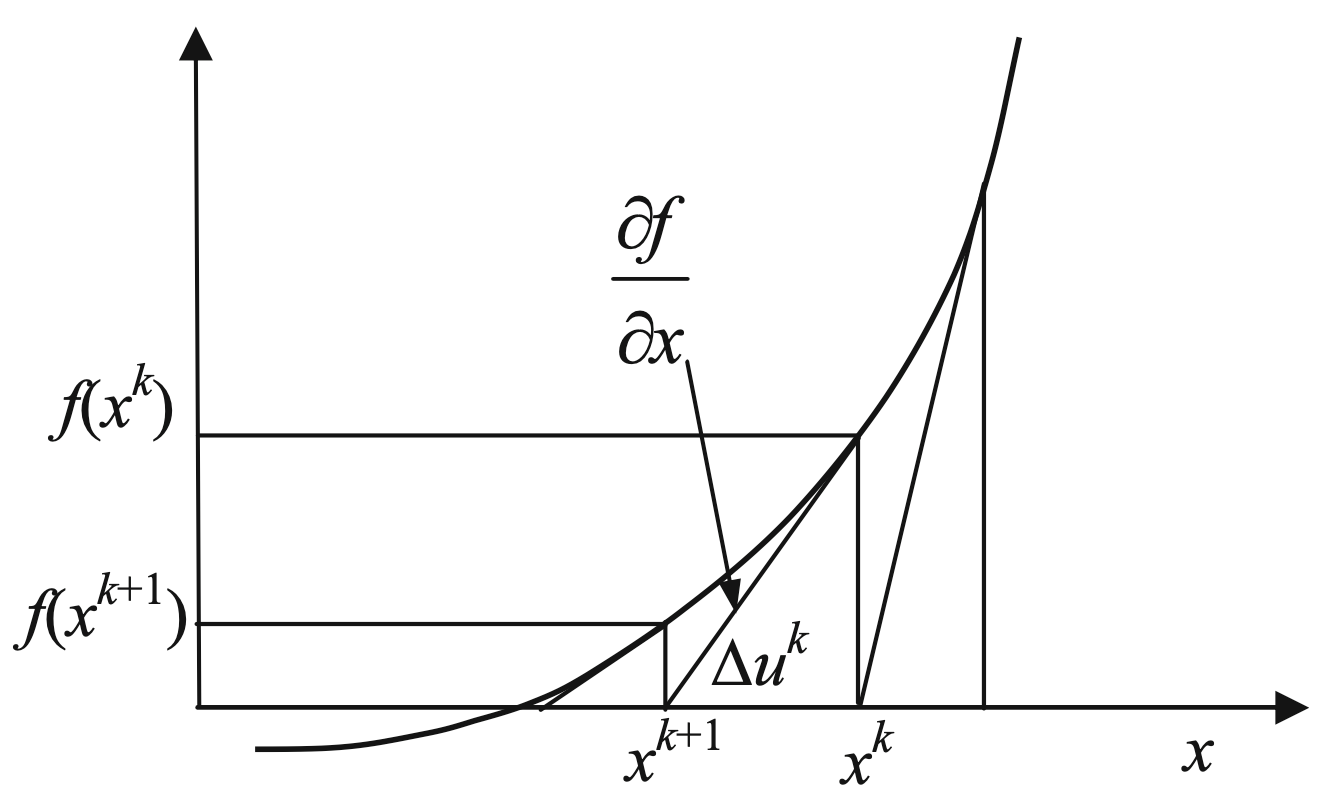
\includegraphics[width=0.45\textwidth]{Imagens/NR.png}
	\caption{Método de Newton–Raphson method para equação não linear, $f=0$}
	\label{fig:NR}
\end{figure}


A equação não linear, Eq.~\eqref{eq:formabilinear} pode ser linearizada usando o mesmo procedimento da Eq.~\eqref{eq:MetodoNR}. Como a forma de carga na Eq.~\eqref{eq:operadorForca} é independente do deslocamento, não é necessário linearizá-la. A linearização da forma de energia na Eq.~\eqref{eq:operadorBilinear} pode ser expressa como:
\begin{equation}\label{eq:LBilinear}
	L[a(\mathbf{u},\mathbf{\bar{u}})] = \iint_{\Omega_0} \Delta \mathbf{S} : \mathbf{\bar{E}} + \mathbf{S} : \Delta \mathbf{\bar{E}} , d\Omega,
\end{equation}
onde $\Delta \mathbf{S}$ é o incremento de tensão e $\Delta \mathbf{\bar{E}}$ é o incremento da variação de deformação. Para o material de St. Venant–Kirchhoff, a relação tensão-deformação é linear, e assim o incremento de tensão pode ser escrito como:
\begin{equation}
	\Delta \mathbf{S} = \frac{\partial \mathbf{S}}{\partial \mathbf{E}} : \Delta \mathbf{E} = \mathbf{D} : \Delta \mathbf{E},
\end{equation}
onde $\mathbf{D}$ é o tensor constitutivo de quarta ordem, e $\Delta \mathbf{E}$ é o incremento da deformação Lagrangiana. Observando que o incremento do gradiente de deformação é $\Delta \mathbf{F} = \nabla_0 \Delta \mathbf{u}$ da Eq.XXX {\color{red} falta uma parte sobre deformações e suas medidas e tensões e suas medidas}, o incremento da deformação Lagrangiana e sua variação podem ser obtidos como:
\begin{equation}
	\Delta \mathbf{E}(\mathbf{u}, \Delta \mathbf{u}) = \text{sym}(\nabla_0 \Delta \mathbf{u}^T \mathbf{F}),
\end{equation}
e
\begin{equation}
	\Delta \mathbf{\bar{E}}(\Delta \mathbf{u}, \mathbf{\bar{u}}) = \text{sym}(\nabla_0 \mathbf{\bar{u}}^T \nabla_0 \Delta \mathbf{u}).
\end{equation}

Assim, a linearização da forma de energia na Eq.~\eqref{eq:LBilinear} pode ser derivada em relação ao deslocamento e sua variação como:
\begin{equation}\label{eq:LBilinearFinal}
	L[a(\mathbf{u},\mathbf{\bar{u}})] = \iint_{\Omega_0} \mathbf{\bar{E}} : \mathbf{D} : \Delta \mathbf{E} + \mathbf{S} : \Delta \mathbf{\bar{E}}  d\Omega = a^*(\mathbf{u}; \Delta \mathbf{u}, \mathbf{\bar{u}}).
\end{equation}

A notação $a^*(\mathbf{u}; \Delta \mathbf{u}, \mathbf{\bar{u}})$ é usada para indicar que a forma depende implicitamente do deslocamento total $\mathbf{u}$ e é bilinear em relação a $\Delta u$ e $\mathbf{\bar{u}}$. O primeiro integrando de $a^*(\mathbf{u}; \Delta \mathbf{u}, \mathbf{\bar{u}})$ na Eq.~\eqref{eq:LBilinearFinal} depende da relação tensão-deformação e é chamado de \emph{rigidez tangente}, semelhante ao termo de rigidez em sistemas lineares. O segundo integrando, contendo o termo de tensão, só aparece em problemas não lineares geométricos e é chamado de \emph{rigidez inicial de tensão}.

Seja o passo de carga atual $t_n$ e o contador de iteração atual $k$. Assumindo que as cargas aplicadas são independentes do deslocamento, a equação incremental linearizada da Eq.~\eqref{eq:formabilinear} é obtida como:

\begin{equation}\label{eq:incrementolinearizado}
	a \left( u^n_k; \Delta u^k, u \right) = \ell \left( u \right) - a \left( u^n_k; u \right), \quad \forall u \in \mathbb{Z}; 
\end{equation}

e o deslocamento total é atualizado usando

\begin{equation}
	u^{n}_{k+1} = u^{n}_{k} + \Delta u^k. \tag{3.76}
\end{equation}

Observe que a equação incremental, Eq.~\eqref{eq:incrementolinearizado}, está na forma de $[K^n_k] \cdot \{ \Delta u^k \} = \{ R^n_k \}$ após discretização usando elementos finitos, o que será discutido na {\color{red}Seção XXXXX}. A Eq.~\eqref{eq:incrementolinearizado} é resolvida iterativamente até que o resíduo se anule, o que significa que a equação não linear original, Eq.~\eqref{eq:formabilinear}, é satisfe
	

\end{document}